%! Author = admin
%! Date = 21.07.2022

% Preamble
\documentclass[11pt]{article}

% Packages
\usepackage{amsmath} % Mathe-Stuff
\usepackage{hyperref} % Links und andere Referenzen

% Für Bilder
\usepackage{graphicx}
\usepackage{amssymb}

\usepackage{lmodern}
\usepackage[ngerman]{babel}

\title{\LaTeX-Tutorial}
\author{Tim Jungk}
\date{ \today }

% Document
\begin{document}

    \maketitle

    \tableofcontents

    \clearpage


    \section{Einleitung}\label{sec:einleitung}

    Diese Anleitung ist bloß als Vorschritt vor der offziellen FHDW-Vorlage zu betrachten und sollte nicht weiter als nötig verfolgt werden. \\
    Im Quellcode sind kleine Formatierungssachen, die man sich anschauen kann. \\

    Ziel dieser Anleitung ist eine lokale \LaTeX-Installation unter Windows zum Laufen zu bekommen.\\
    Am Ende sollte diese Anleitung ohne Probleme kompiliert werden können.\\

    Es werden drei Komponenten installiert:

    \begin{itemize}
        \item \LaTeX - Um das Dokument zu kompilieren
        \item Git - Um den Quellcode zu versionieren
        \item Intellij - Um den Quellcode zu bearbeiten
    \end{itemize}


    \section{Installation}\label{sec:installation}

    \begin{center}
        Hinweis: Die Installation bezieht sich auf Windows, bei Fragen zu Unix-Systemen gerne ansprechen.
    \end{center}

    \subsection{MikTex}\label{subsec:miktex}

    \href{https://miktex.org/download}{MikTex Download}, einmal anklicken
    \\
    Auf der Webseite unter: Windows >> Installer >> Download einmal runterladen und öffnen.
    \\
    Die Standard-Einstellungen sollten passen.
    Man wird gefragt, wie fehlende Pakete installiert werden sollen Dort >>On the fly<< oder >>Never Ask<< auswählen.
    \\
    Dann öffnet man die Miktex Konsole, wenn dies nicht automatisch passiert, einfach in Windows danach suchen.
    % include image
    \begin{center}
        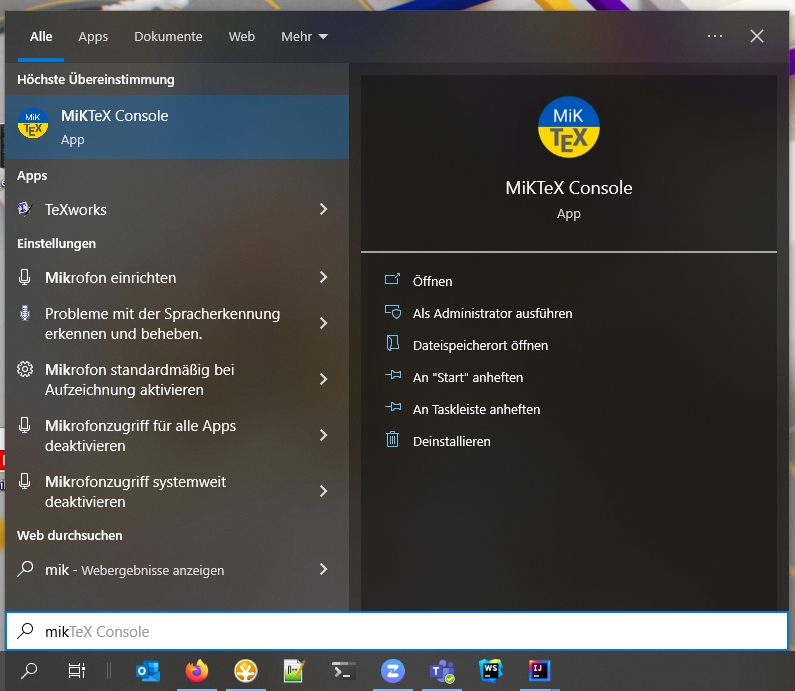
\includegraphics[width=6cm]{resources/mik-tex}
    \end{center}

    \subsubsection{Konfiguration nach dem Update}

    MikTex leitet einen da gut durch.
    Nach dem Öffnen, öffnet sich eine Meldung, das noch keine Updates installiert wurden.
    Der Knopf ist rot umrandet.
    Diesen drückt man.

    \subsection{GIT (optional, aber sehr empfehlenswert)}\label{subsec:git}
    \href{https://git-scm.com/download/win}{https://git-scm.com/download/win} öffnen.
    >>64-bit Git for Windows Setup<< anklicken und der Installation ganz normal folgen.

    Als Einführung empfiehlt sich \href{https://www.youtube.com/watch?v=hwP7WQkmECE&ab_channel=Fireship}{\underline{dieses Video}}.

    Auf weitere Funktionen sei in Eigenrecherche zu stoßen, kurz das wichtigste.

    \begin{center}
        \begin{tabular}[h]{|l|l|}
            \hline
            git commit & Die Dateien lokal committen = Quasi neue Version erstellen               \\
            \hline
            git push   & Die Dateien auf z.B.\ GitHub pushen  = Quasi neue Version veröffentlichen \\
            \hline
        \end{tabular}
    \end{center}

    \subsection{IntelliJ IDEA}\label{subsec:intellij-idea}

    Wenn nicht schon geschehen, dann IntelliJ herunterladen.
    Die Community Edition ist vollkommen ausreichend.
    \href{https://www.jetbrains.com/idea/download/#section=windows}{IntelliJ Download}

    \subsubsection{Repository herunterladen}

    IntelliJ öffnen und >>Get from VCS<< anklicken. \\

    \begin{center}
        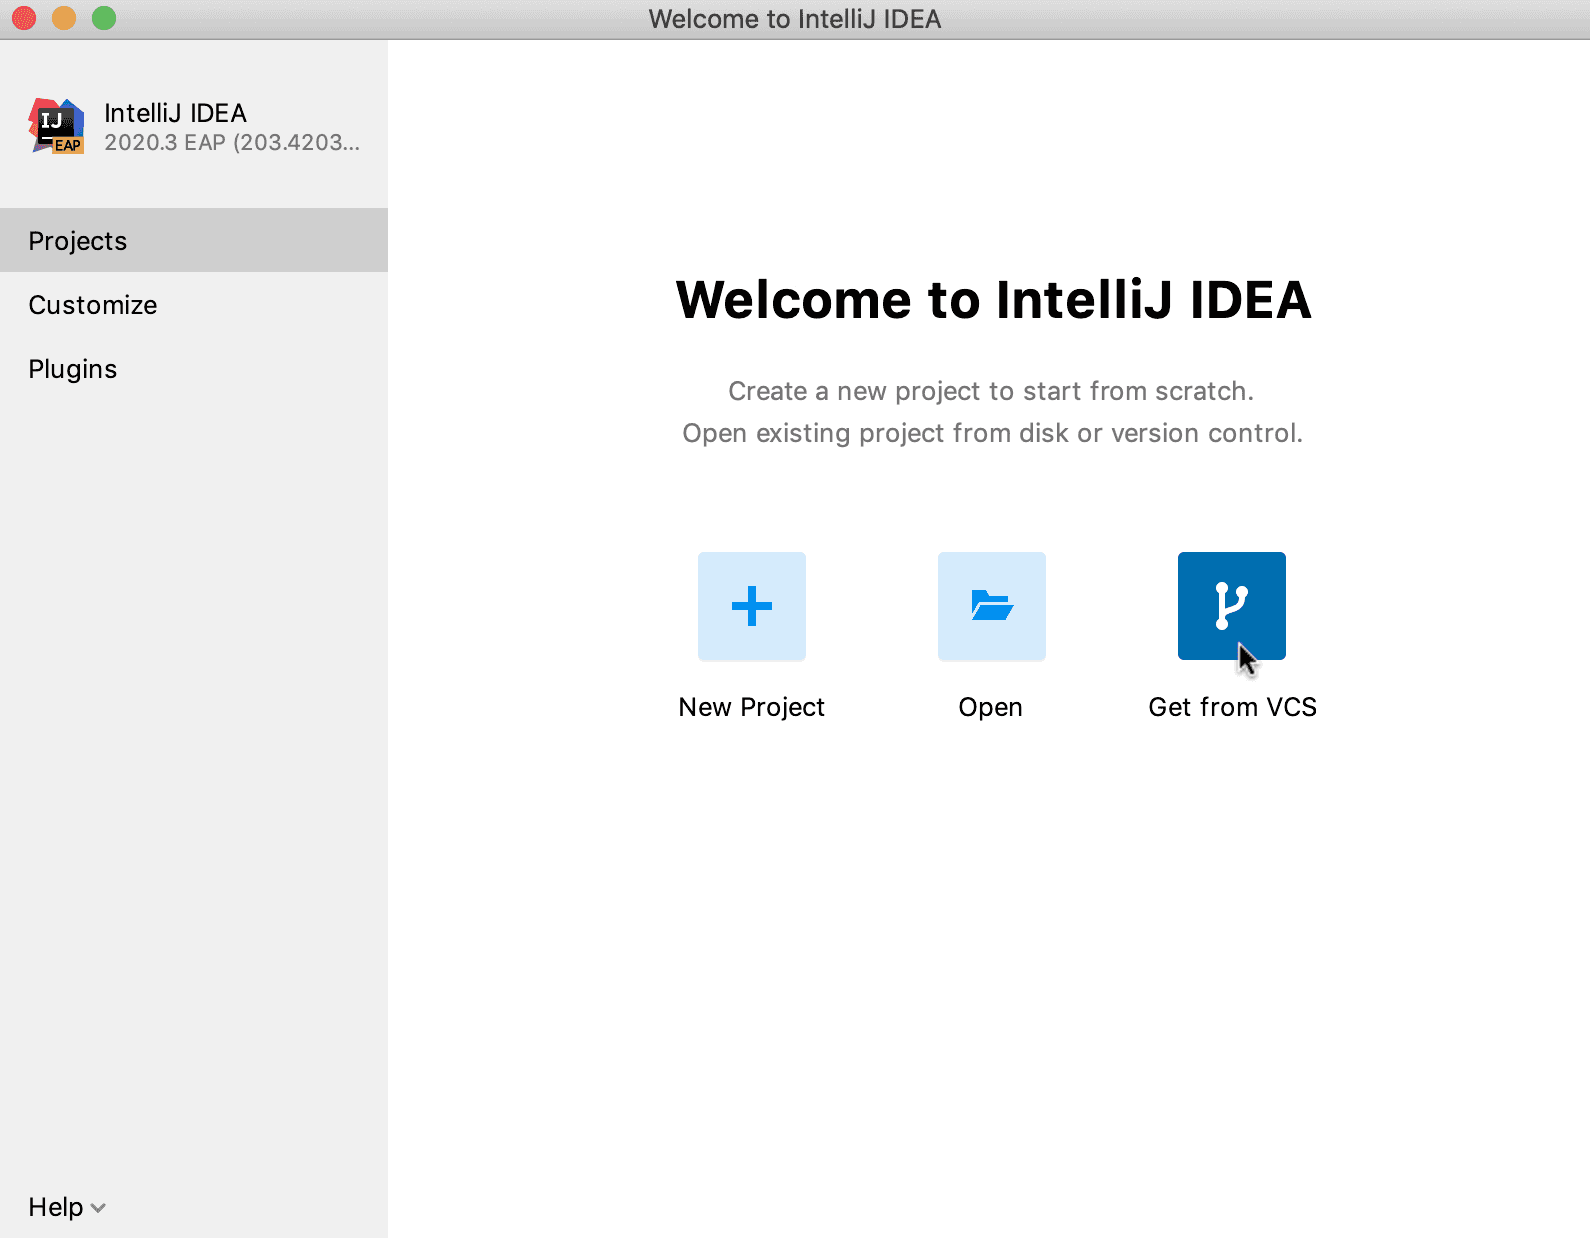
\includegraphics[width=\textwidth]{resources/intellij}
    \end{center}

    Dort folgenden Link einfügen: \underline{https://github.com/TimJ0212/Tutorial} \\

    Einmal laden und dann sollte unten links etwas stehen à la "Download Required Plugins", da einmal auf Ok drücken.

    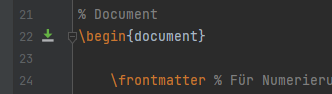
\includegraphics[width=5cm]{resources/int-comp}

    Danach sollte sich in Zeile 23 ein Symbol zeigen, wenn nicht, dann einfach IntelliJ neustarten. \\

    Das Symbol einmal anklicken, als Ergebnis sollte im Ordner Out, an der linken Seite, eine \textbf{out.pdf} zeigen, diese einfach öffnen.


    \section{Workflow}\label{sec:workflow}

    Es lohnt sich sehr auf IntelliJ als Git-GUI-Client zu setzten.
    Dafür klickt man einfach unten oder auf der Linken Seite auf >>Git<< oder >>Commit<<, dort kann man die veränderten Dateien dann committen.

    \section{Praxisarbeit beginnen}\label{sec:praxisarbeit-beginnen}

    \begin{enumerate}
        \item \href{https://www.overleaf.com/read/yrndghycwxgb}{\underline{Vorlage}} öffnen
        \item oben links auf >>Menu<< und dann >>Source<< klicken.
        \item Den Ordner irgendwo abelgen.
        \item  In IntelliiJ oben auf File >> Open und dann den Ordner raussuchen. \\
        \item Praxisarbeit kann beginnen!
    \end{enumerate}

\end{document}